% 2011_zhejiang_liberal_q7_optB: cuboid + slanted top block
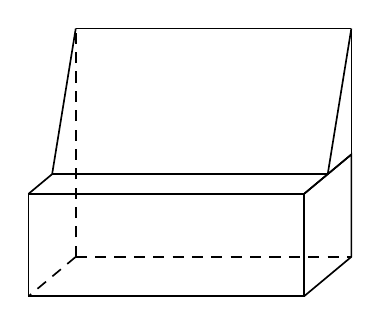
\begin{tikzpicture}[x=1cm,y=1cm,font=\normalsize,
  solid edge/.style={solid,line width=.6pt},
  hidden edge/.style={dashed,line width=.6pt,dash pattern=on 4pt off 3pt}]
\coordinate (F1) at (0,0);
\coordinate (F2) at (3.5,0);
\coordinate (F3) at (3.5,1.3);
\coordinate (F4) at (0,1.3);
\coordinate (H0) at (0.6,0.5);
\coordinate (B2) at (4.1,0.5);
\coordinate (B3) at (4.1,1.8);
\coordinate (T1) at (0.3,1.55);
\coordinate (T2) at (3.8,1.55);
\coordinate (U1) at (0.6,3.4);
\coordinate (U2) at (4.1,3.4);
\draw[solid edge] (F1) -- (F2) -- (F3) -- (F4) -- cycle;
\draw[solid edge] (F2) -- (B2) -- (B3) -- (F3);
\draw[solid edge] (F4) -- (F3);
\draw[solid edge] (F3) -- (B3);
\draw[solid edge] (T1) -- (T2);
% top slanted block front face: T1-U1-U2-(F3 side)
\draw[solid edge] (F4)--(T1)--(U1);
\draw[solid edge] (U1) -- (U2);
\draw[solid edge] (U2) -- (T2);
\draw[solid edge] (U2)--(B3);
\draw[solid edge] (T1) -- (T2);
\draw[hidden edge] (H0) -- (F1);
\draw[hidden edge] (H0) -- (B2);
\draw[hidden edge] (H0) -- (U1);


\end{tikzpicture}
